\section{Introduction}

\begin{figure}[t]
    \centering
    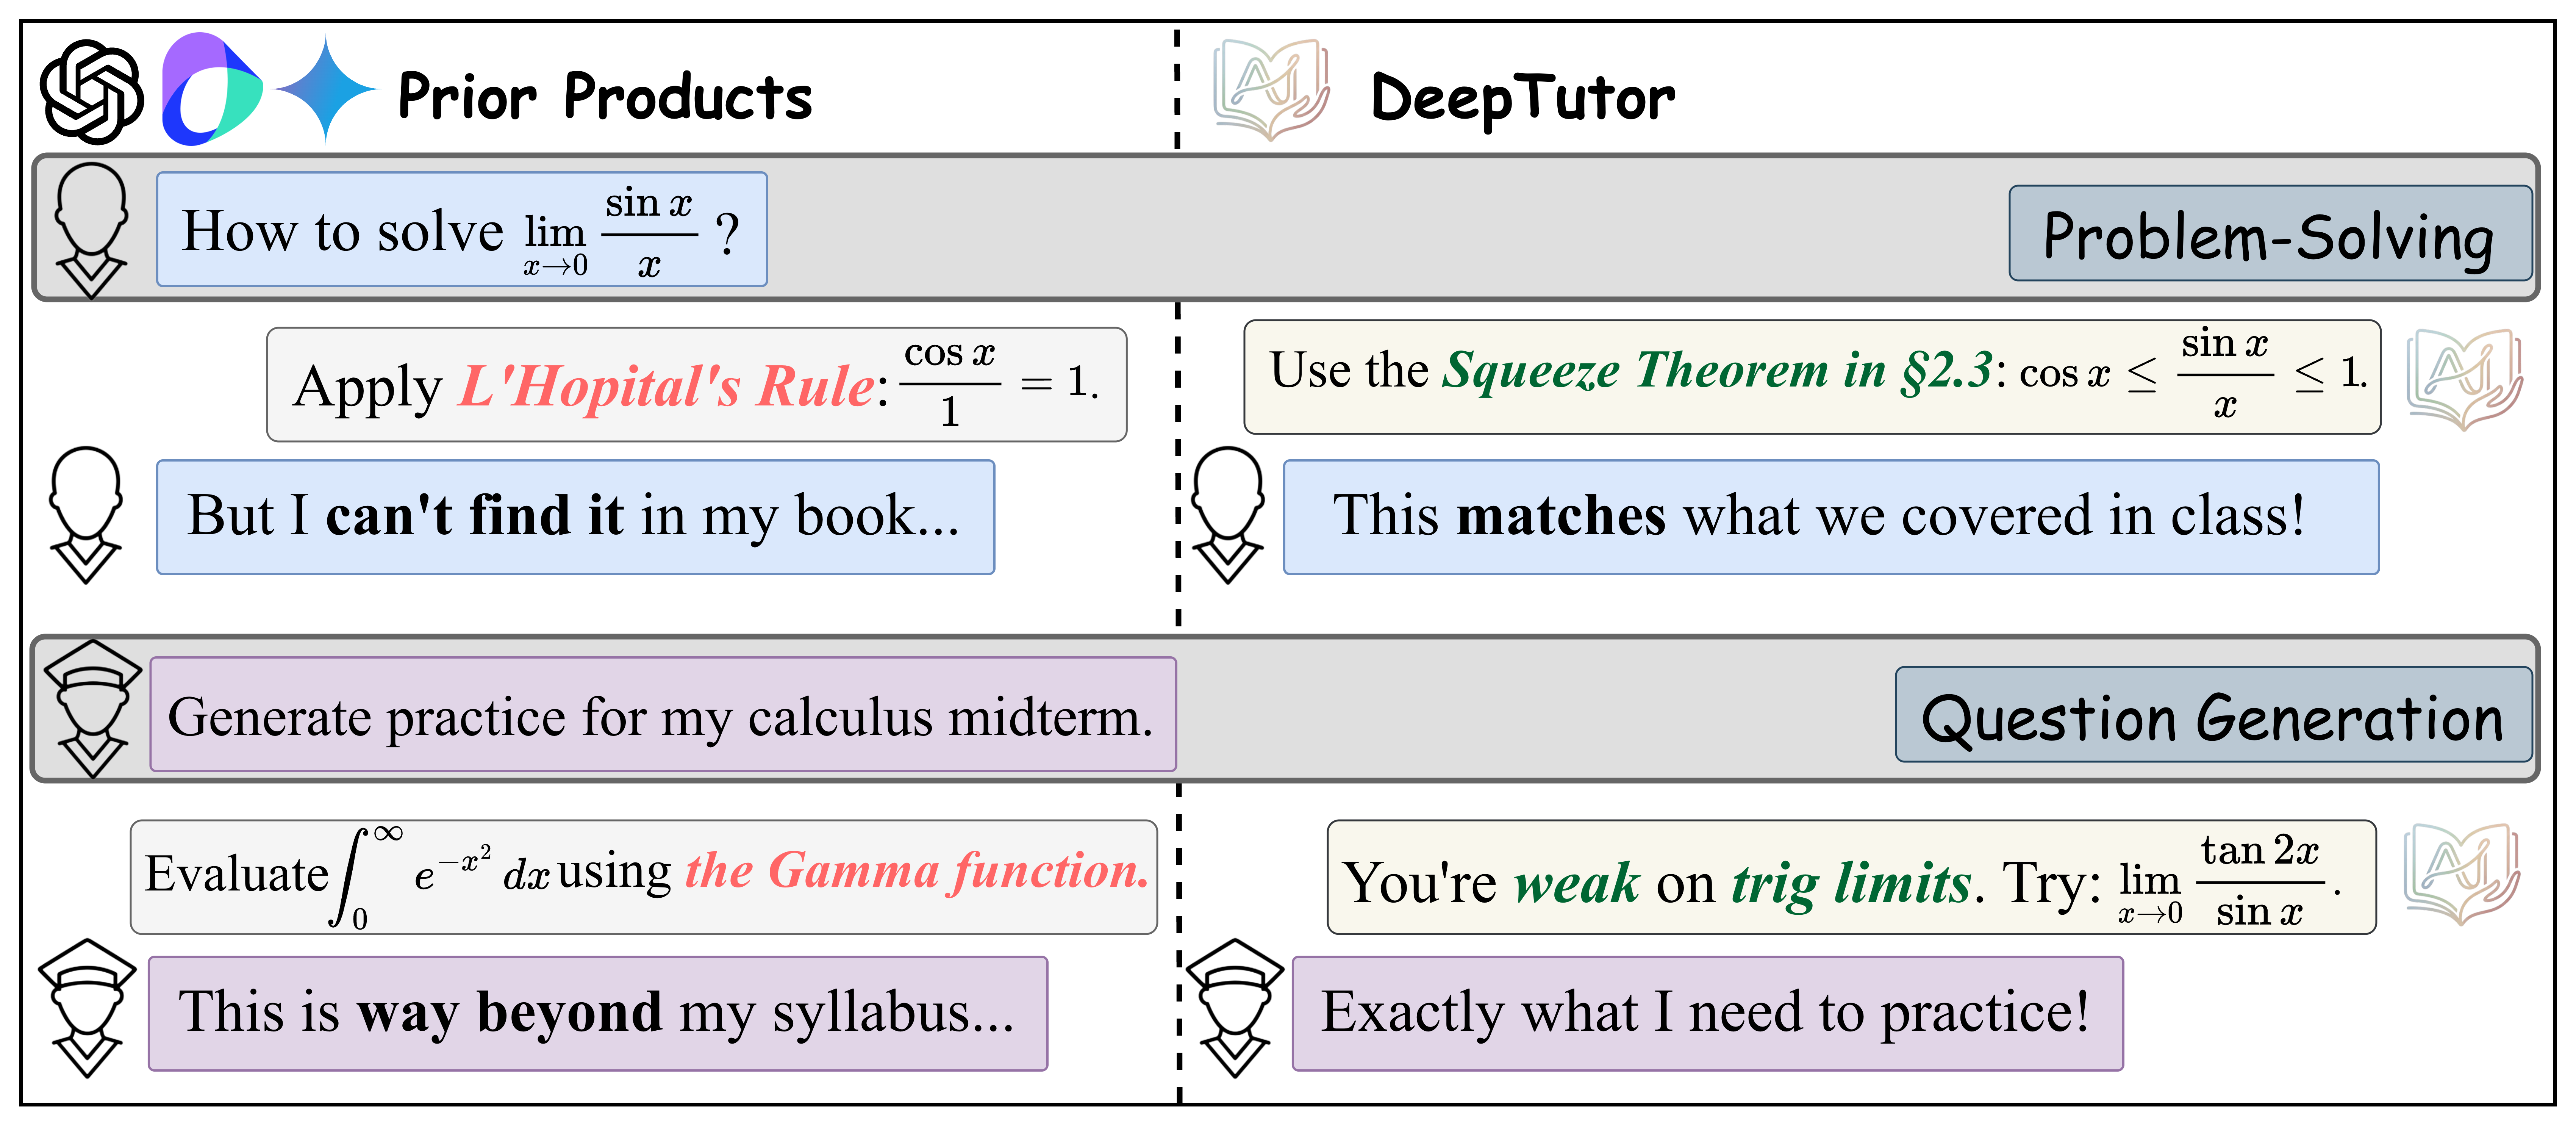
\includegraphics[width=\columnwidth]{figures/compare-ver1.png}
    \caption{Comparison of \textit{prior LLM products} and \textsc{DeepTutor}. Existing products provide generic answers regardless of the learner's background; \textsc{DeepTutor} adapts both problem-solving explanations and generated practice to match the student's syllabus, knowledge level, and specific weaknesses exposed during conversation.}
    \label{fig:compare}
\end{figure}

Education is among the most promising real-world applications of large language models (LLMs).
An effective human tutor does far more than supply correct answers--they diagnose misconceptions, scaffold explanations to the learner's level, and continuously pose targeted practice that turns weaknesses into strengths \citep{letourneau2025systematicreviewaidriven}.
While LLMs exhibit impressive fluency in educational dialogues, replicating this tightly integrated set of pedagogical skills within a unified, adaptive system remains an open challenge \citep{chu-etal-2025-llm}.

Existing approaches tackle fragments of this challenge in isolation. As illustrated in Figure~\ref{fig:compare}, the question generation of existing LLM systems rarely calibrates difficulty to the individual learner. Though SOTA LLMs demonstrate strong STEM reasoning abilities, they often tend to solve the question in a general way as they were trained. 
Question generation, on the other hand, often fails to fit the student's syllabus.
Personalized educational platforms track coarse skill inventories rather than the fine-grained reasoning traces that reveal \textit{how} a student errs.
Meanwhile, retrieval-augmented generation (RAG) often lacks consideration for the adaptive, guided explanations that effective tutoring demands.

We argue that the missing ingredient is a \textit{closed interactive loop}: weaknesses exposed during problem solving should directly shape which questions are generated next, while the learner's performance on those questions should, in turn, refine the model that informs future explanations.
This requires operationalizing personalization into measurable mechanisms, such as calibrating question difficulty based on diagnosed weaknesses and adapting explanation depth to the learner's proficiency.
Realizing such a loop requires (i)~a structured memory that captures fine-grained interaction histories rather than scalar skill scores, and (ii)~a unified tutoring system whose modules share and continuously update that memory.

To address these problems, we propose \textsc{DeepTutor} that unifies both problem solving and question generation within a hybrid personalization framework. 
For problem solving, we utilize an \textit{investigation--solving--writing} pipeline that decomposes complex queries, executes multi-step tool-augmented reasoning, and synthesizes citation-grounded explanations.
For question generation, a \textit{critic-guided generate--validate loop} iteratively proposes and verifies difficulty-calibrated practice items.
Moreover, both pipelines are unified through a hybrid personalization engine that couples static knowledge grounding with \textit{trace forest}, a dynamic structured memory that records multi-resolution interaction traces and employs specialized memory agents to continuously refine an evolving learner profile---creating the closed tutoring cycle where every interaction personalizes the next.

Our main contributions are as follows:
\begin{itemize}[nosep,leftmargin=*]
  \item We propose \textsc{DeepTutor}, an agentic tutoring framework that, to the best of our knowledge, is among the first to unify tool-augmented problem solving, critic-guided question generation, and long-term structured memory into a closed interactive loop.
  \item We introduce \textit{trace forest}, a hierarchical memory architecture in which specialized agents collaboratively maintain a fine-grained, evolving learner model from multi-resolution interaction traces.
  \item We construct \textsc{TutorBench}, a benchmark of 100 knowledge-base-grounded learner profiles paired with a student simulator for first-person interactive evaluation. Experiments on TutorBench and five standard reasoning benchmarks show that \textsc{DeepTutor} substantially outperforms various baselines, providing insights for the future shape of personalized tutoring systems.
\end{itemize}
